\documentclass[3pt, sigconf, nonacm]{acmart}
\usepackage{booktabs} % For formal tables
\usepackage{float}
\usepackage{enumitem}
\usepackage{textcomp}
\usepackage{caption}
\usepackage{titlesec}


% Remove the conference information
\settopmatter{printacmref=false} % Removes citation information below abstract
\renewcommand\footnotetextcopyrightpermission[1]{} % Removes footnote with conference information in first column

\renewcommand{\normalsize}{\fontsize{8.5}{10}\selectfont}
\normalsize

\titleformat{\section}
  {\normalfont\fontsize{10}{13}\bfseries}{\thesection}{1em}{}

\begin{document}

\title{Natural Language Project Report}
\subtitle{Natural Language 2024/25 | Group 3}

\author{Gonçalo Carvalho}
\affiliation{
  \institution{ist199227}
  \city{~}
  \country{~}
}

\author{Leonor Carvalho}
\affiliation{
    \city{~}
  \country{~}
  \institution{ist199623}
}

\author{Guilherme Leitão}
\affiliation{
  \institution{ist199951}
  \city{~}
  \country{~}
}
\renewcommand{\shortauthors}{Natural Language | Group 2}



\maketitle

\section{Models}
% (3 points) this section contains a clear description of your model(s) and all the preprocessing done (if applicable)
\setlength{\parindent}{0pt}

In order to enhance the dataset for training, the following preprocessing steps were carried out in sequence:

\begin{enumerate}
    \item \textbf{Concatenation of text fields}: Different combinations of the text fields were tested, concatenating them into a single feature to provide a comprehensive representation of the data; the best results were obtained by combining the \textit{from}, \textit{title} and \textit{director} with the \textit{plot} field.
    \item \textbf{Synonym-based data augmentation}: To address class imbalance, we used the    \textsc{NLPAug} library~\cite{ma2019nlpaug} to perform data augmentation through synonym replacement, substituting words in sentences from minority classes with their synonyms.
    \item \textbf{Data normalization}: We replaced missing values with empty strings, removed special characters and digits, and converted all text to lowercase.
    \item \textbf{Expansion of Contractions}: Contractions in short texts were expanded to their full forms for improved clarity.
    \item \textbf{Part-Of-Speech Tagging and Lemmatization}: The Python library \textsc{NLTK}~\cite{bird2009natural} and the WordNet\textregistered ~database~\cite{miller-1994-wordnet} were used for POS tagging, followed by lemmatization.
    This ensures that words are reduced to their base forms despite syntactic variations.
    \item \textbf{Removal of Stop Words}: Common stop words were removed to focus on the most informative terms. The English stop words list from the \textsc{NLTK} library~\cite{bird2009natural} was used, and a minimum document frequency threshold was defined for additional filtering.
\end{enumerate}

For feature extraction, we used a count vectorizer and a TF-IDF transformer to convert the preprocessed data into numerical vectors.
Two models from the \textsc{sklearn}~\cite{scikit-learn} library were used to classify the train set:

\begin{itemize}
    \item \textbf{Support Vector Machine (SVM)}: Discriminative classifier that maximizes the margin between classes.
    \item \textbf{Multinomial Naive Bayes (MNB)}: Probabilistic classifier for text; assumes independent features.
\end{itemize}


\section{Experimental Setup and Results}
% : in this section you should detail your experimental setup (evaluation measures, datasets used, development set, parameters, etc.) and present your model(s) results. These should be presented in a table, considering accuracy (general results, and also the results obtained by genre); you should also present a comprehensive confusion matrix. As previously said, the expected genres of the given test set are not provided (test_just_plots.txt), so you should create your own test(s) set(s) from the training set and report the results on your own test(s) 

%\subsection{Experimental Setup}
We used \textsc{GridSearchCV}~\cite{lavalle2004relationship} from \textsc{sklearn} library to systematically evaluate various combinations of hyperparameter values (by cross-validation) and determine the optimal configuration that maximizes accuracy.

\begin{itemize}
    \item \textbf{Dataset}: Stratified split (per genre) \textit{train.txt} into training (90\%) and test (10\%) sets.
    \item \textbf{Evaluation Measures}: Used accuracy, precision, recall, F1-measure and confusion matrices; calculated per-genre accuracy.
    \item \textbf{Best Model Parameters}: TF-IDF with a maximum of 10000 features, an ngram range between 1 and 5 tokens (found after manual fine-tuning - Fig.~\ref{fig:ngram}), sublinear tf scanning and the following sets of stop-words:
    \begin{figure}[h]
        \centering
        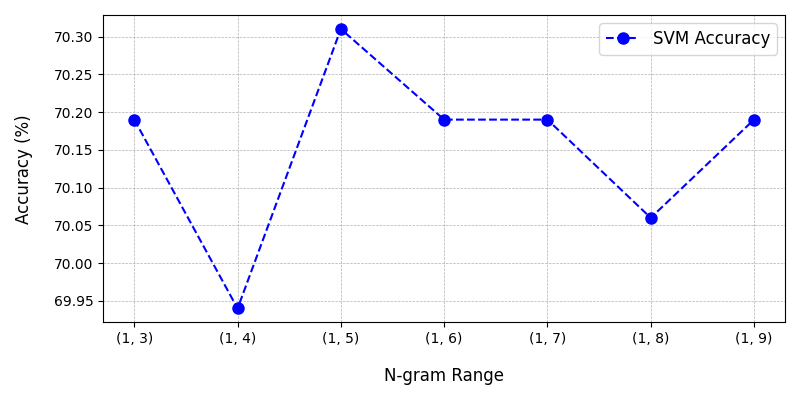
\includegraphics[width=1.0\linewidth]{images/ngram.png}
        \caption{\footnotesize N-gram Range.}
        \Description{~}
        \label{fig:ngram}
    \end{figure}
    \begin{itemize}
        \item \textbf{English}: we calculated every word's DF score and removed only those with a frequency higher than 15\%. Later, as can be seen in Fig.~\ref{fig:threshold}, we tested different thresholds to find the optimal value to be 0\% (meaning all stop-words were removed).
        \begin{figure}[h]
            \centering
            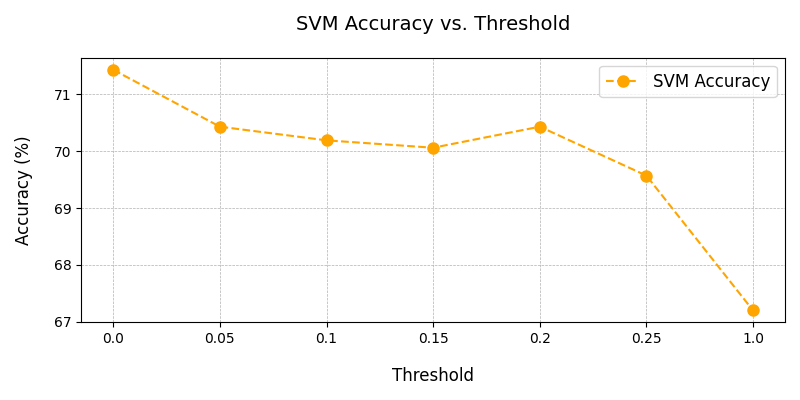
\includegraphics[width=1.0\linewidth]{images/threshold.png}
            \caption{\footnotesize Document Frequency Threshold.}
            \Description{~}
            \label{fig:threshold}
        \end{figure}

        \item \textbf{Custom}: even though they are not stop-words by definition, we added specific $genre$ words —  ``action'', ``animation'', ``comedy'', ``crime'', ``horror'' and ``western'' - to the stop-words list and removed them from the dataset to reduce "$genre$ contamination".
    \end{itemize}
    For the models, we applied hyperparameter tuning to the following parameters, having achieved the respective optimal values:
    \begin{itemize}
        \item \textbf{SVM}: $kernel = sigmoid; C = 1; class\_weight = None$
        \item \textbf{MNB}: $alpha = 0.1; fit\_prior = True$
    \end{itemize}
\end{itemize}

%\subsection{Results}

Table~\ref{tab:accuracy} presents the overall best mean cross-validation accuracy. 
\begin{table}[h]
\centering
\caption{\footnotesize Overall Accuracy per Model.}
\renewcommand{\arraystretch}{0.8} % Reduce row height
\begin{tabular}{lcc}
\toprule
\textbf{Model} & \textbf{Accuracy (\%)} \\
\midrule
Support Vector Machine & 70.31 \\
Multinomial Naive Bayes & 64.97 \\
\bottomrule
\end{tabular}
\label{tab:accuracy}
\end{table}


As we can see, the best model was the SVM, henceforth every analysis will be based on its results.

Table~\ref{tab:per-genre-metrics} shows the metrics for each genre.

\begin{table}[h]
\centering
\caption{\footnotesize Per-Genre Metrics.}
\label{tab:per-genre-metrics}
\renewcommand{\arraystretch}{1.0} % Reduce row height
\begin{tabular}{lccc}
\toprule
\textbf{Genre} & \textbf{Precision} & \textbf{Recall} & \textbf{F1-Score} \\
\midrule
Action & 0.68 & 0.65 & 0.66 \\
Animation & 0.86 & 0.80 & 0.83 \\
Comedy & 0.66 & 0.64 & 0.65 \\
Crime & 0.53 & 0.56 & 0.54 \\
Drama & 0.61 & 0.72 & 0.66 \\
Horror & 0.87 & 0.83 & 0.85 \\
Romance & 0.57 & 0.48 & 0.52 \\
Sci-Fi & 0.85 & 0.52 & 0.65 \\
Western & 0.94 & 0.98 & 0.96 \\
\bottomrule
\end{tabular}
\end{table}


Table~\ref{tab:per-iteration} illustrates the accuracy and F1-score per model with a modified preprocessing hyperparameter.

\begin{table}[h]
\centering
\caption{\footnotesize Per-Hyperparameter Metrics.}
\label{tab:per-iteration}
\resizebox{\columnwidth}{!}{ % Adjust table to fit column width
\begin{tabular}{@{}lcccccc@{}}
\toprule
\textbf{Metrics} & \textbf{Best} & \textbf{No} & \textbf{``Plot''} & \textbf{Keeping} & \textbf{Keeping} & \textbf{No} \\
& \textbf{Model} & \textbf{Lemmatize} & \textbf{Only} & \textbf{$genre$ Words} & \textbf{Stopwords} & \textbf{Augmentation} \\
\midrule
Accuracy (\%)   & 70.31 & 69.19 & 67.70 & 69.81 & 66.83 & 67.58 \\
F1-Score        & 0.70  & 0.69  & 0.68  & 0.70  & 0.67  & 0.67  \\
\bottomrule
\end{tabular}
}
\end{table}

Fig.~\ref{fig:confusion matrix} shows the confusion matrix for the best model, which represents the optimal combination of hyperparameters from \textsc{GridSearchCV}.


\begin{figure}[h]
    \centering
    \includegraphics[width=1.0\linewidth]{images/confusion_matrix.png}
    \caption{\footnotesize Confusion Matrix for SVM.}
    \Description{~}
    \label{fig:confusion matrix}
\end{figure}

\section{Discussion}
% (5 points): here, I expect you to show me that you have properly analysed the dataset and the obtained outputs (not just by looking at statistics or a confusion matrices). I really want you to look at the plots that resulted in errors. Explain the most common errors (examples are mandatory)
%We augmented the data to increase samples within minority classes while preserving the relative distribution between genres. The 'No Augmentation' model scored lower than the best model, suggesting that data scarcity could be a significant constraint.


As shown in Fig.~\ref{fig:genre word distribution}, most $genre$ words appeared with higher frequency in $genres$ not matching their own (the effect is scaled with data augmentation). These words, being directly associated with the classification task of the model, can lead the model to predict the class of the word rather than the actual class of the movie. This means that the word may be interpreted outside of its semantic context, leading to inaccurate predictions.

With this in mind, we decided to remove these words from the dataset. However, we decided not to remove "sci-fi" due to tokenization issues related to the hyphen. Additionally, we kept the word "romance" because we noticed a significant drop in precision for this class after removing it. The model struggled to interpret the concept of a romance film, and retaining the word improved performance. This suggests that "romance" is an essential word for describing this type of movie, as romance movies are generally not so closely associated with other genres. Instead, it is other genres that often incorporate romantic elements, highlighting the uniqueness of romance as a genre.

Including the word "romance" allows the model to more easily recognize the category of romantic films, thereby improving the accuracy of predictions. This experience underscores the importance of considering semantic context and word associations when dealing with text classification in natural language processing.



%Focusing only on plot results in lower accuracy and F1-score, which indicates that other text elements are also crucial for accurate predictions.



\begin{figure}
    \centering
    \includegraphics[width=1.0\linewidth]{images/genre word distribution.png}
    \caption{\footnotesize Distribution of $genre$ words.}
    \Description{~}
    \label{fig:genre word distribution}
\end{figure}

The SVM model outperformed MNB in overall accuracy, likely due to its effectiveness in high-dimensional spaces like TF-IDF vectors.


Common misclassifications occurred between similar genres:

\begin{itemize}
    \item \textbf{Drama vs. Romance}: We think this common mislabelling be due to the fact that in both genres plots featuring relationships facing challenges are common as well as other common themes.
    \item \textbf{Drama vs. Comedy}: We believe this mislabelling might occur due to the existence of comedic dramas, or dramas in which an unusual or humorous character or situation are present.
\end{itemize}

\textbf{Examples of Misclassified Plots}

\begin{itemize}
    \item \textbf{Plot}: ``Wealthy friends are entangled in a dispute that strains their children's engagement through deceit, love and the revelation of the truth, they reconcile and allow their children to marry.'' \textbf{Actual Genre}: Drama  \textbf{Predicted}: Romance
    \item \textbf{Plot}: `` A virginal sixth-former delivering groceries for the local supermarket, is more interested in seducing the local girls.'' \textbf{Actual Genre}: Drama  \textbf{Predicted}: Comedy
\end{itemize}

\section{Future Work}
%(1 point): if more time was given to you, explain what you would do to improve your system

\begin{itemize}
    \item \textbf{Hyperparameter tuning}: adjusting the number of synonyms used for data augmentation and fine-tuning the amount of generated data 
    \item \textbf{Data augmentation techniques}: paraphrasing (back translation, text expansion and entity substitution) or GANs
    \item \textbf{Latent Dirichlet Allocation} to identify underlying themes or topics present in the text data.
    \item \textbf{Deep Learning Models}: LSTMs or Transformers for better semantic understanding.

\end{itemize}
\clearpage
\bibliographystyle{IEEEtran}
\bibliography{references}
\end{document}